\section{Voice recognition}\label{sec:voice}

Today's neural networks work on algorithmically very complex, yet 
intuitive tasks. These objectives can be categorized into two main 
classes: \emph{supervised} and \emph{unsupervised}. 
The trend shows that sample labeling slavery becomes unfavored, 
because human-resource for classifying and evaluating tasks is getting more expensive.
Therefore classical supervised learning is getting less attention over time. 
Still understanding how these models (should) work is essential and 
demonstrating via the simplest examples leads to some interesting case 
studies. In the following an informal introduction presents results of 
such experiments.

\paragraph{Technical background.} 
For the sake of readability the detailed implementation of the perceptron 
framework is excluded from this work (although can be found in 
\url{~/tree/master/demo/audio} at the GitHub repository of my implementation \cite{DV}). 
The writing assumes basic knowledge in linear algebra, the model will be described in the following manner:
 
\begin{figure}
	\centering
	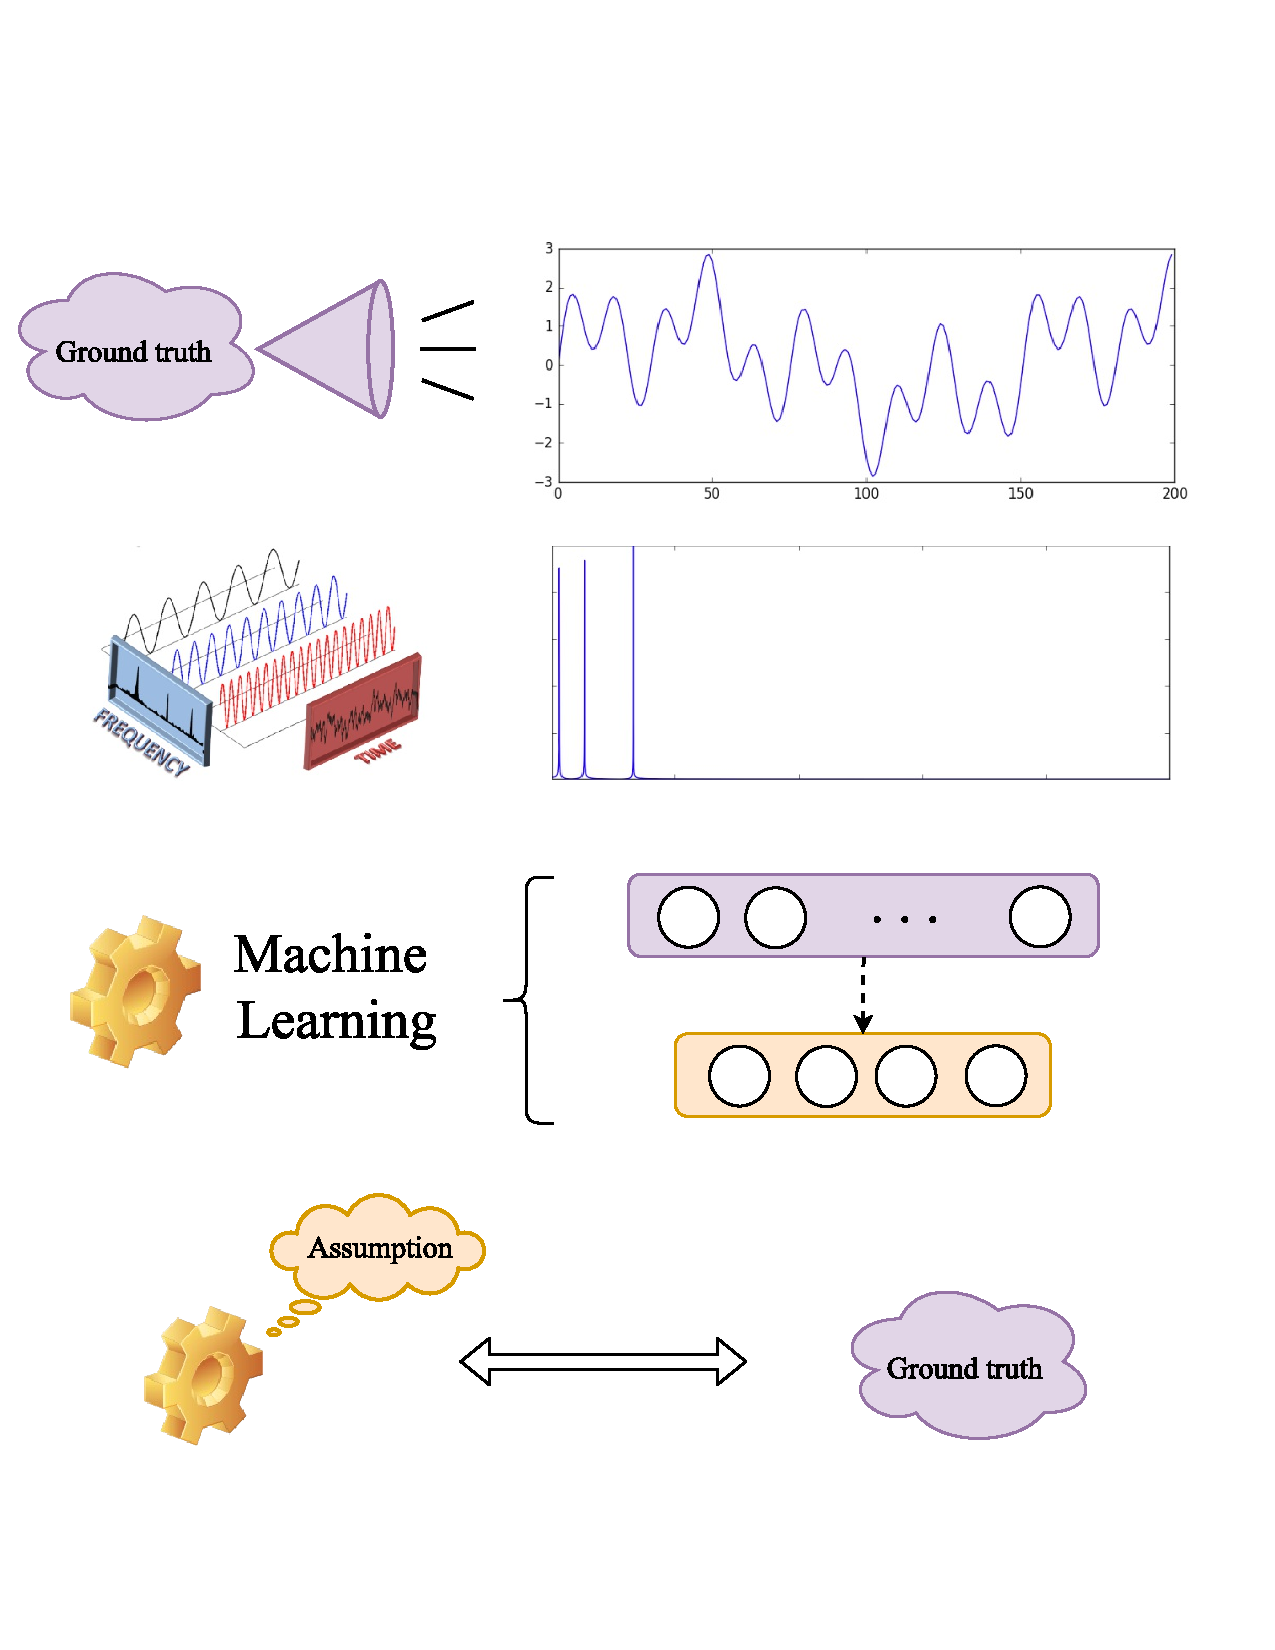
\includegraphics[width=0.9\textwidth]{workflow.pdf}
	\caption{
	The basic conception of voice recognition: 
	the original message is first expressed in physical waveforms which may introduce a lot of noise in real life. 
	After recording, the wave in time domain, it is transferred to \emph{frequency domain} that 
	tells which frequencies were dominant in the captured signal sample.
	According to nature's biological systems in this form the same information can be better processed.
	}
	\label{fig:workflow}
\end{figure}
For a given network $\mathcal{F}$ and fixed length input $x$ the system's assumption, the output, is computed as $y=\mathcal{F}(x)$, where $y$ is a fixed length vector.
$\mathcal{F}$ can be seen as a \emph{black box}, that takes $dim(x)$ information, somehow processes it and - if $\mathcal{F}$ is trained correctly it returns the class of $x$. Practically $dim(y)=|\{\textrm{classes}\}|$ - therefore $y$ represents the network's confidence on each class (detailed explanation \ref{eq:softmax}). 

\subsection{Separating sine waves}
After defining the model, the first implementation should be able to classify the low- and high-pitch samples. For starting let the low-pitch sample, $\mathbf{x^1}$ be a sine function with frequency $F1$, and high-frequency sample $\mathbf{x^2}$, a sine with frequency $F2$. 
For mimicking the nature's living systems (especially the inner ear), the sample is transformed to frequency domain with an algorithm called \emph{N-point Fast Fourier Transform} \cite{welch1967use}. 
\paragraph{Fourier Transform in a nutshell.} Basically the result of the transformation tells which frequencies were dominant in the time domain, which is a better clue for both the living, and the machines too. 
The architecture will be two perceptrons in the same layer. 
For each $\mathbf{x_i}$ they have different weights, which helps them decide when to turn on, and when to output lower value. 
For details see Figure \ref{fig:N500}. 
For the script which was used to produce the figures check out \cite{DV}.

\begin{figure}
	\centering
	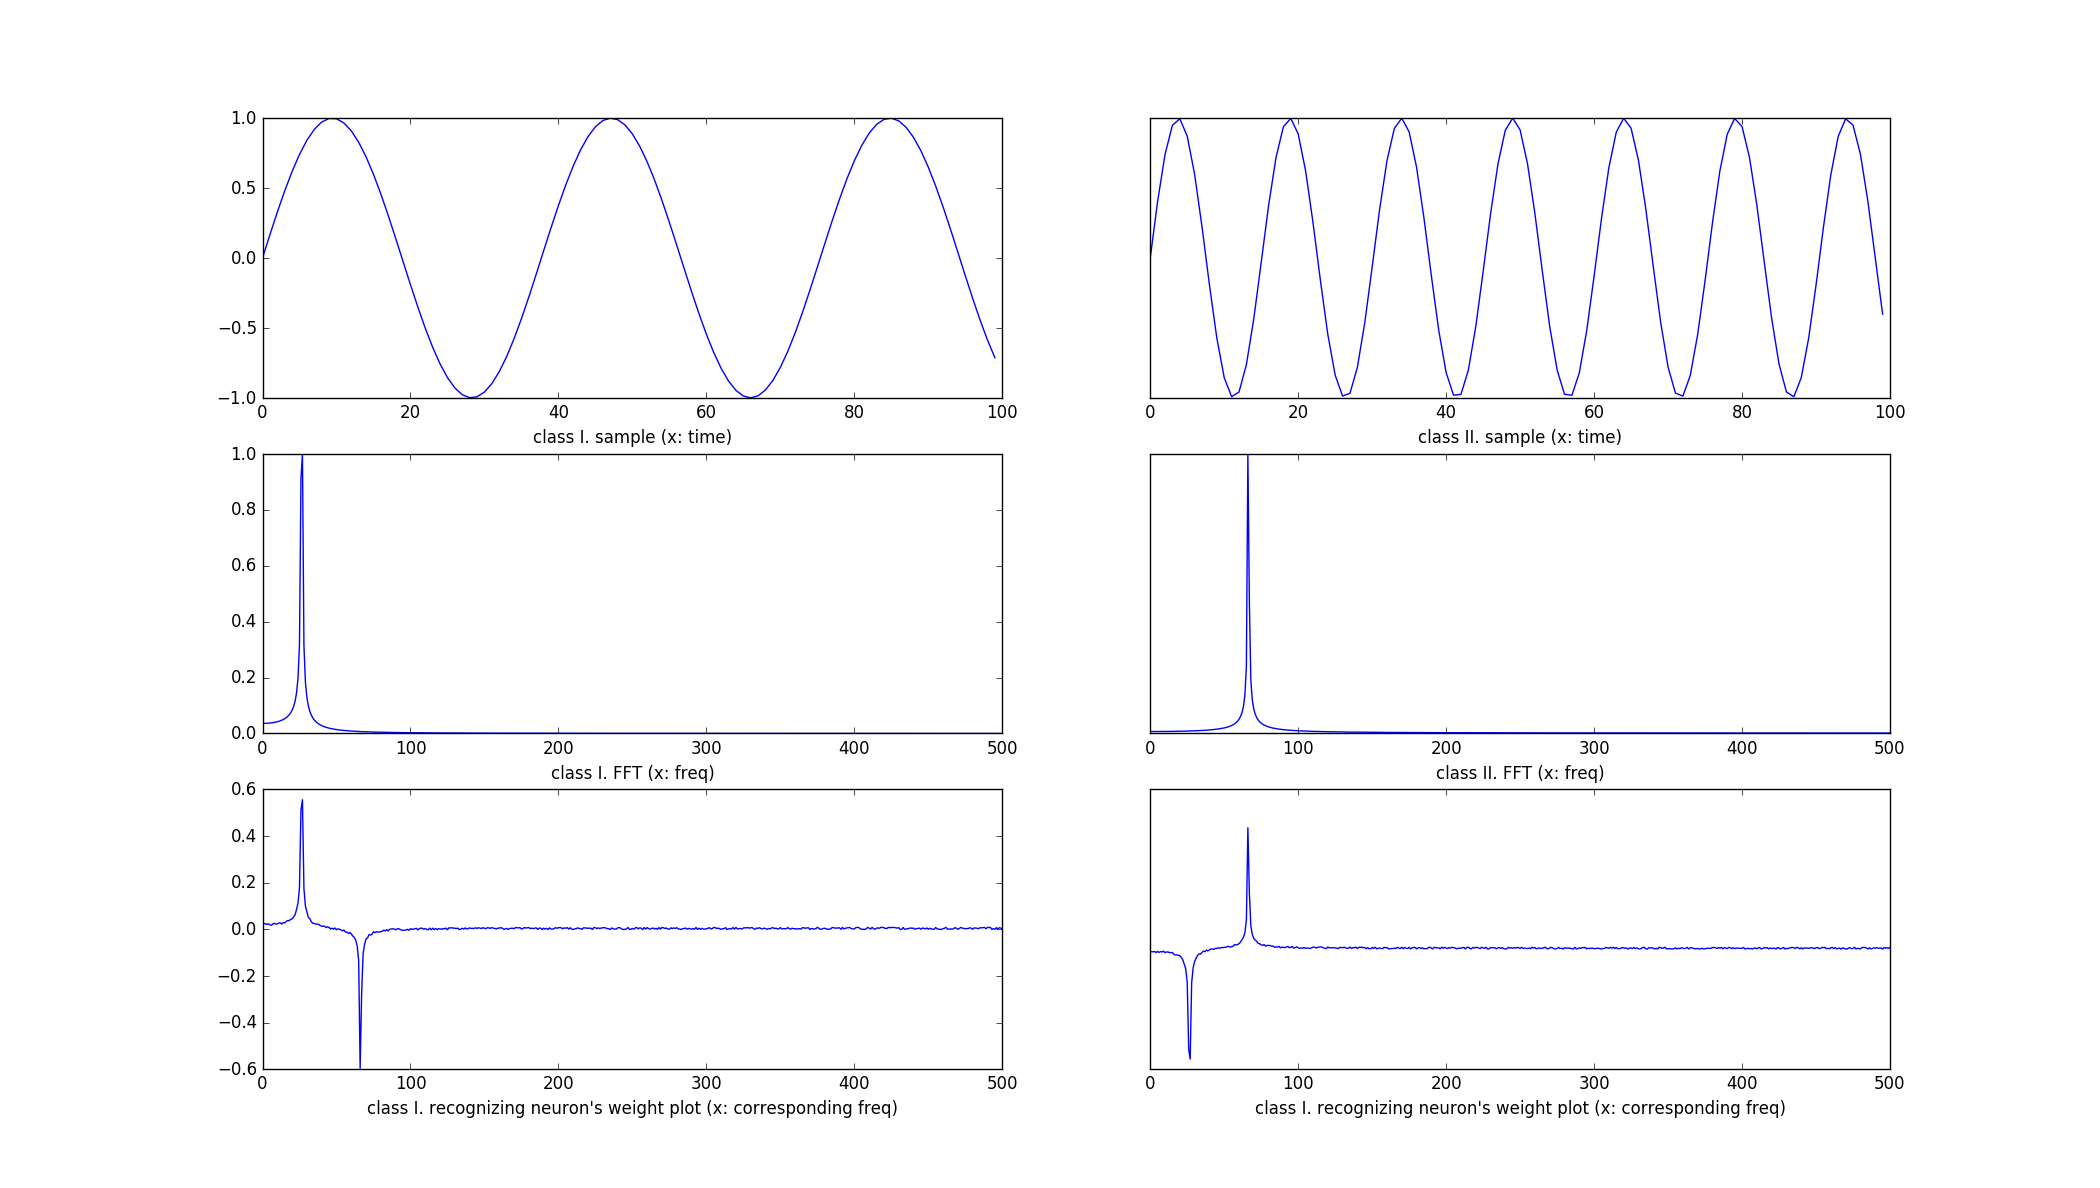
\includegraphics[width=0.8\textwidth]{N500-L2e-1.png}
	\caption{On the first row the original sample is shown in time domain.
	 On the second row the N-FFT of it. On the last row the plot of the 
	 weights of the corresponding perceptron. 
	 The first feature to 
	 recognize, that each perceptron learned that not just to turn on for 
	 the corresponding input sample, but to output negative values when 
	 samples of the opposite class are shown to the network. 
	 The network 
	 was initialized with Gaussian random noise with mean at 0 and 
	 deviation $1/2$, and trained with mini-batch size 1, learning rate $
	 \eta=0.5$, \emph{regularization} factor $\lambda=0.1$ for 10 epoch 
	 with \emph{cross-likelihood} error function}
	
	\label{fig:N500}
\end{figure}

\paragraph{Varying the precision of the Fourier Transform, N.}
For such arbitrary cases, where no noise is added to the signal, larger precision is unnecessary, for validation check Figure \ref{fig:N5000}, \ref{fig:N50}. However the importance of choosing the right N should not be underestimated: in environments with loss \emph{Signal-to-Noise ratio} it is advised to use high \emph{sampling rate}, and large $N$, however for real-time applications it is a trade-off between quality and speed, because the computation complexity for this architecture is $\mathcal{O}(N^2)$, therefore choosing too large N results in slow processing.

\begin{figure}
	\centering
	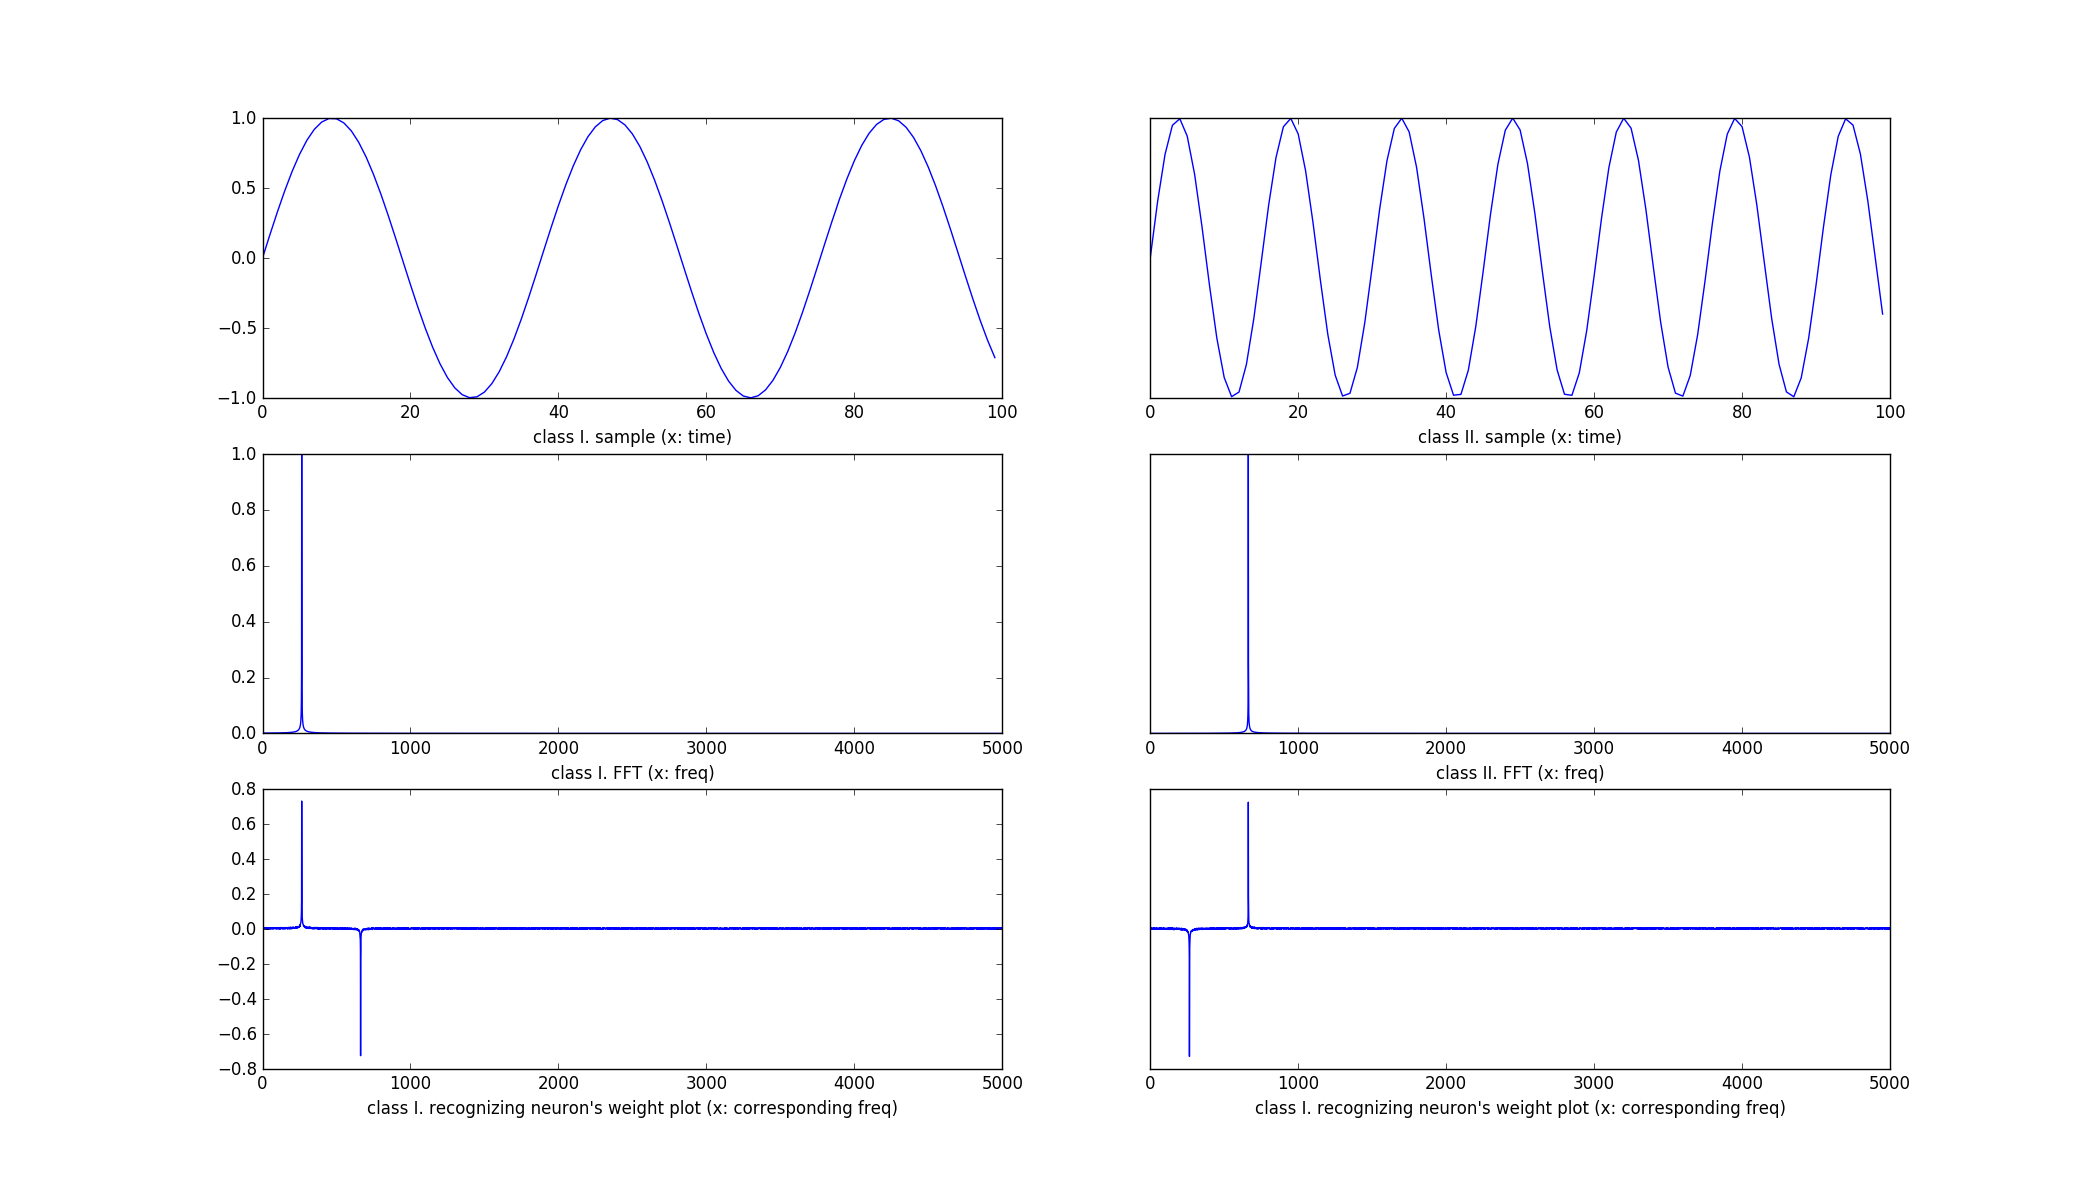
\includegraphics[width=0.8\textwidth]{N5000-L2e-1.png}
	\caption{The network's initialization and training parameters are identical to the network depicted on Figure \ref{fig:N5000}, only the transform precision is increased from $N=500$ to $N=5000$ resulting in more narrow spikes corresponding to the recognized frequency}
	
	\label{fig:N5000}
\end{figure}


\begin{figure}
	\centering
	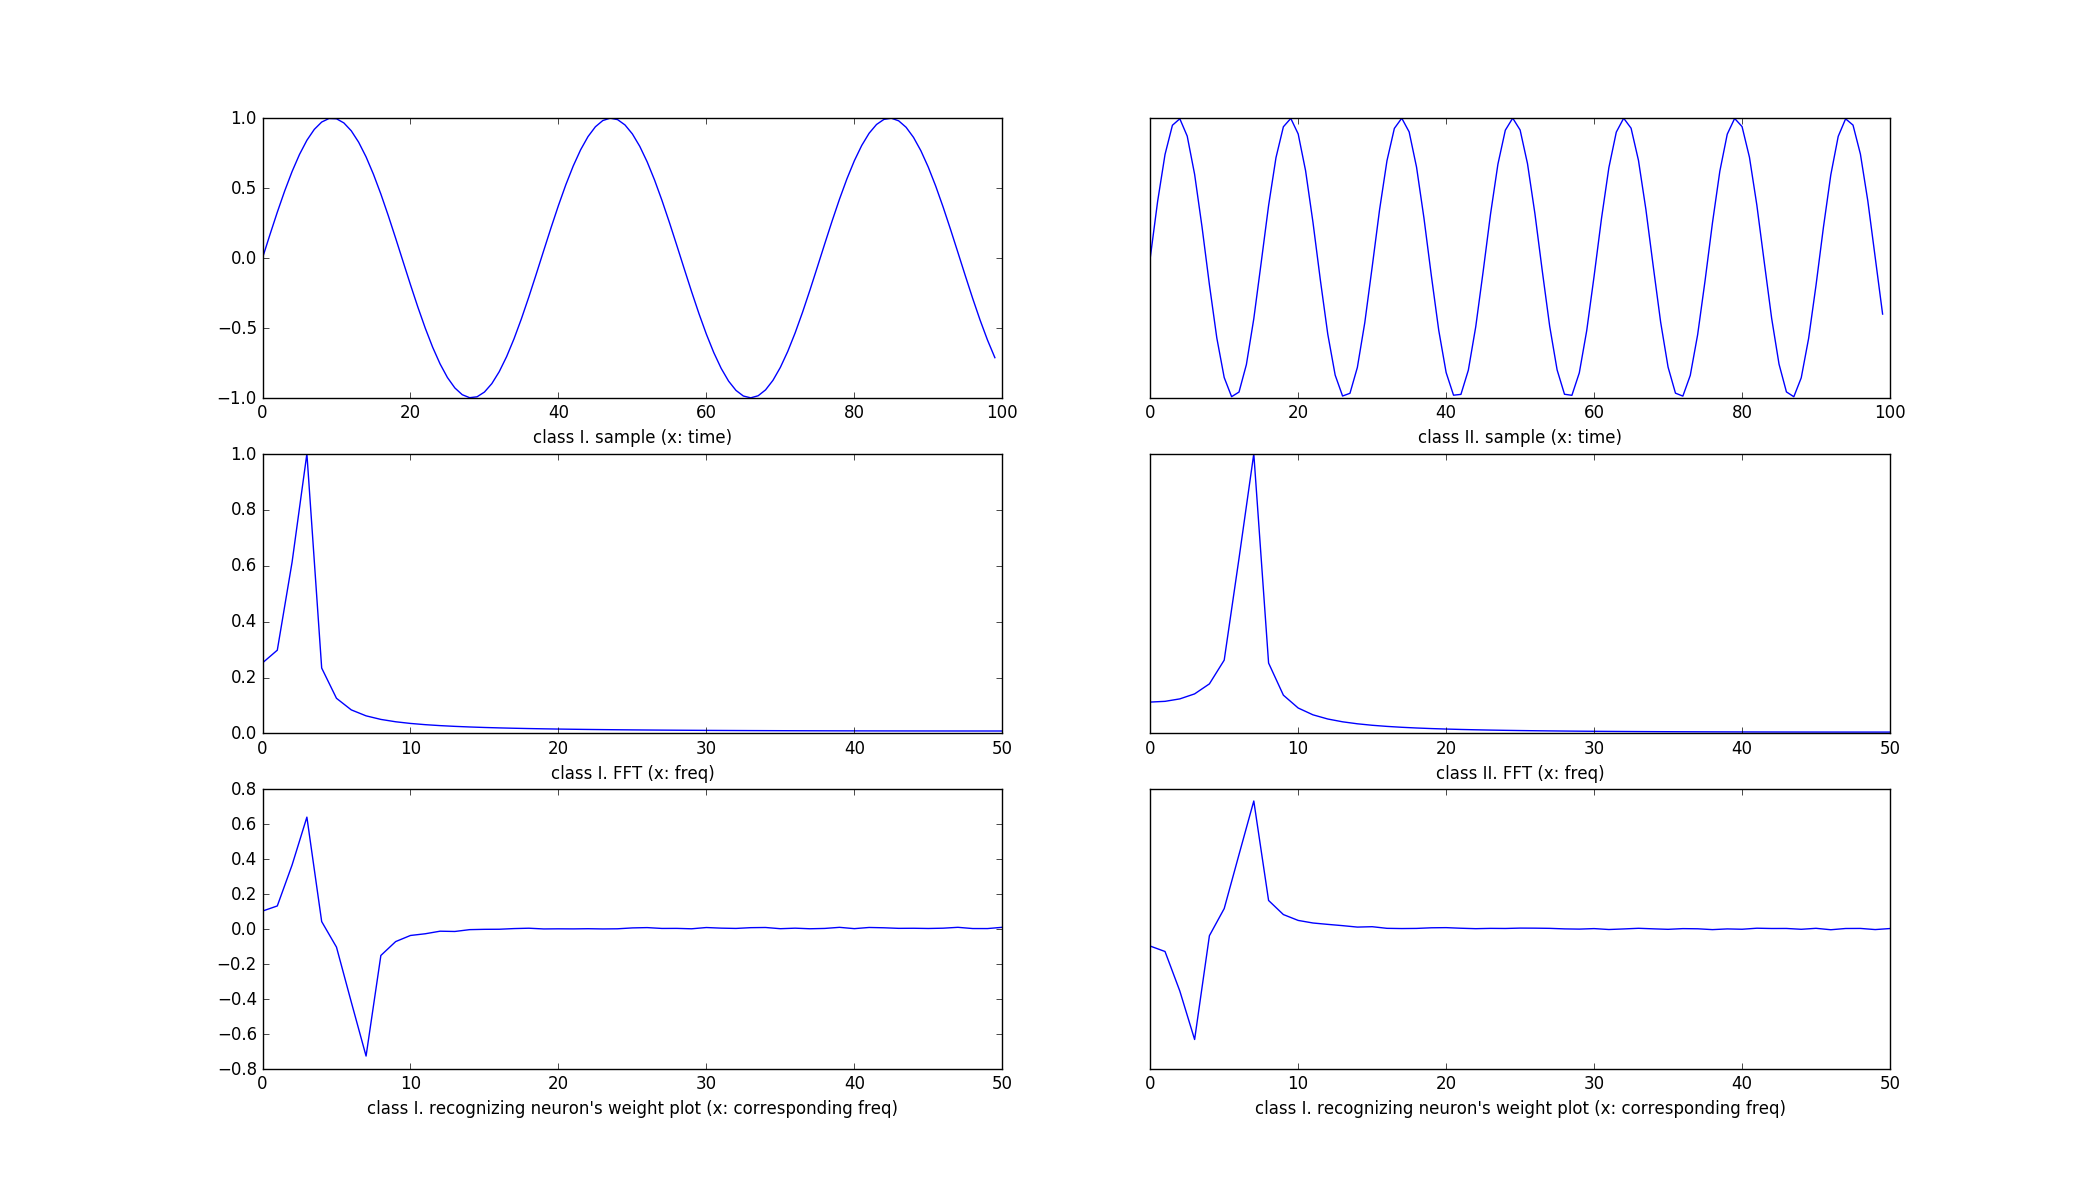
\includegraphics[width=\textwidth]{N50-L2e-1.png}
	\caption{The network's initialization and training parameters are identical to the network depicted on Figure \ref{fig:N500}, only the transform precision is decreased from $N=500$ to $N=50$ resulting in more shallow spikes corresponding to the recognized frequency}
	
	\label{fig:N50}
\end{figure}

\begin{figure}
	\centering
	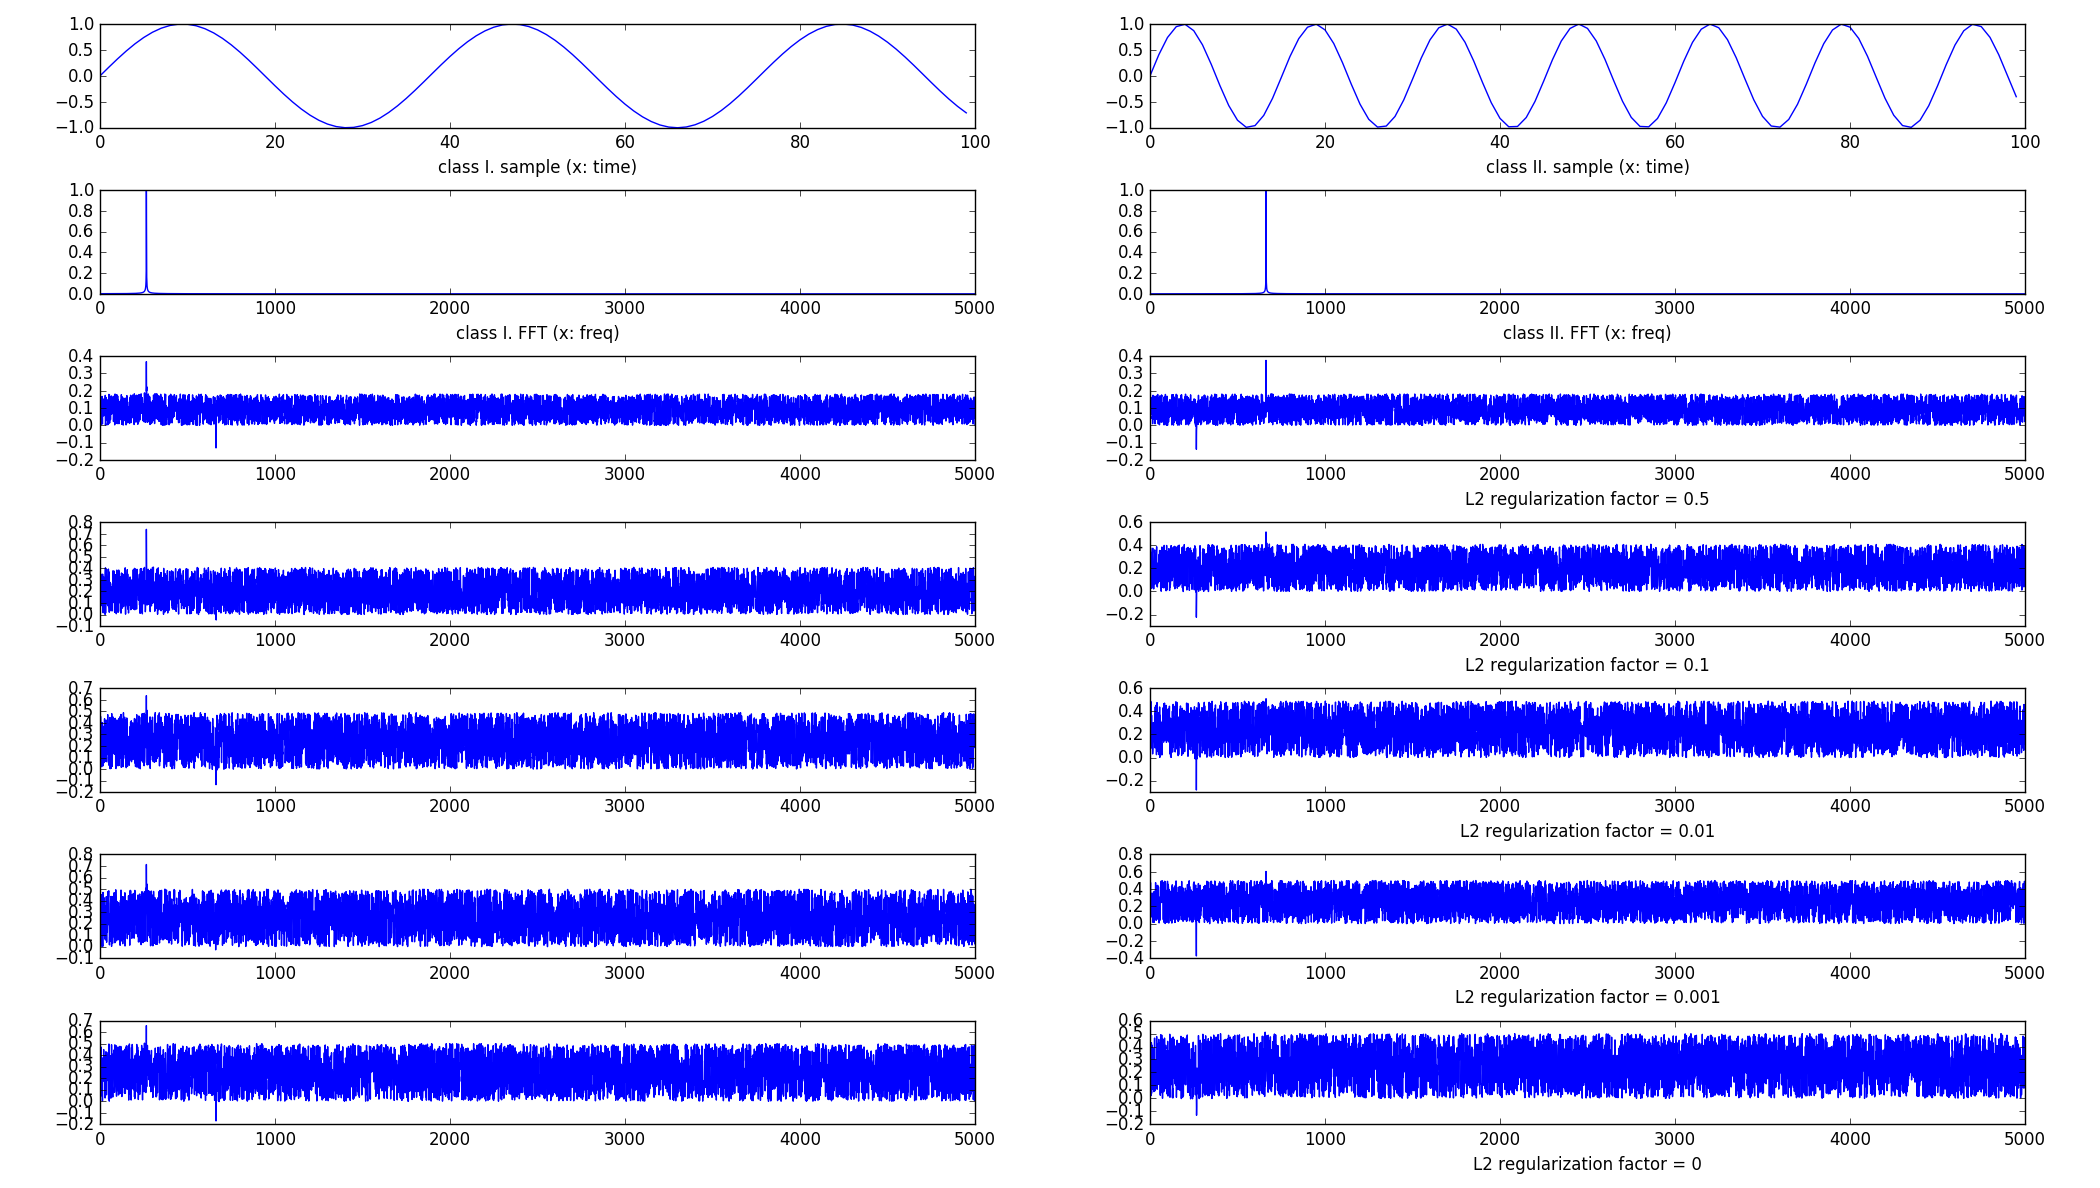
\includegraphics[width=\textwidth]{L2_factor_plot--5epoch.png}
	\caption{After the third row the figure depicts independently, identically initialized and trained networks detailed in Figure \ref{fig:N500}, only the regularization factor $\lambda$ is decreased from $0.5$ to $0.0001$ resulting in more noisy weight plot. Still the  corresponding weights' magnitude are outstanding}
	
	\label{fig:reg}
\end{figure}

\begin{figure}
	\centering
	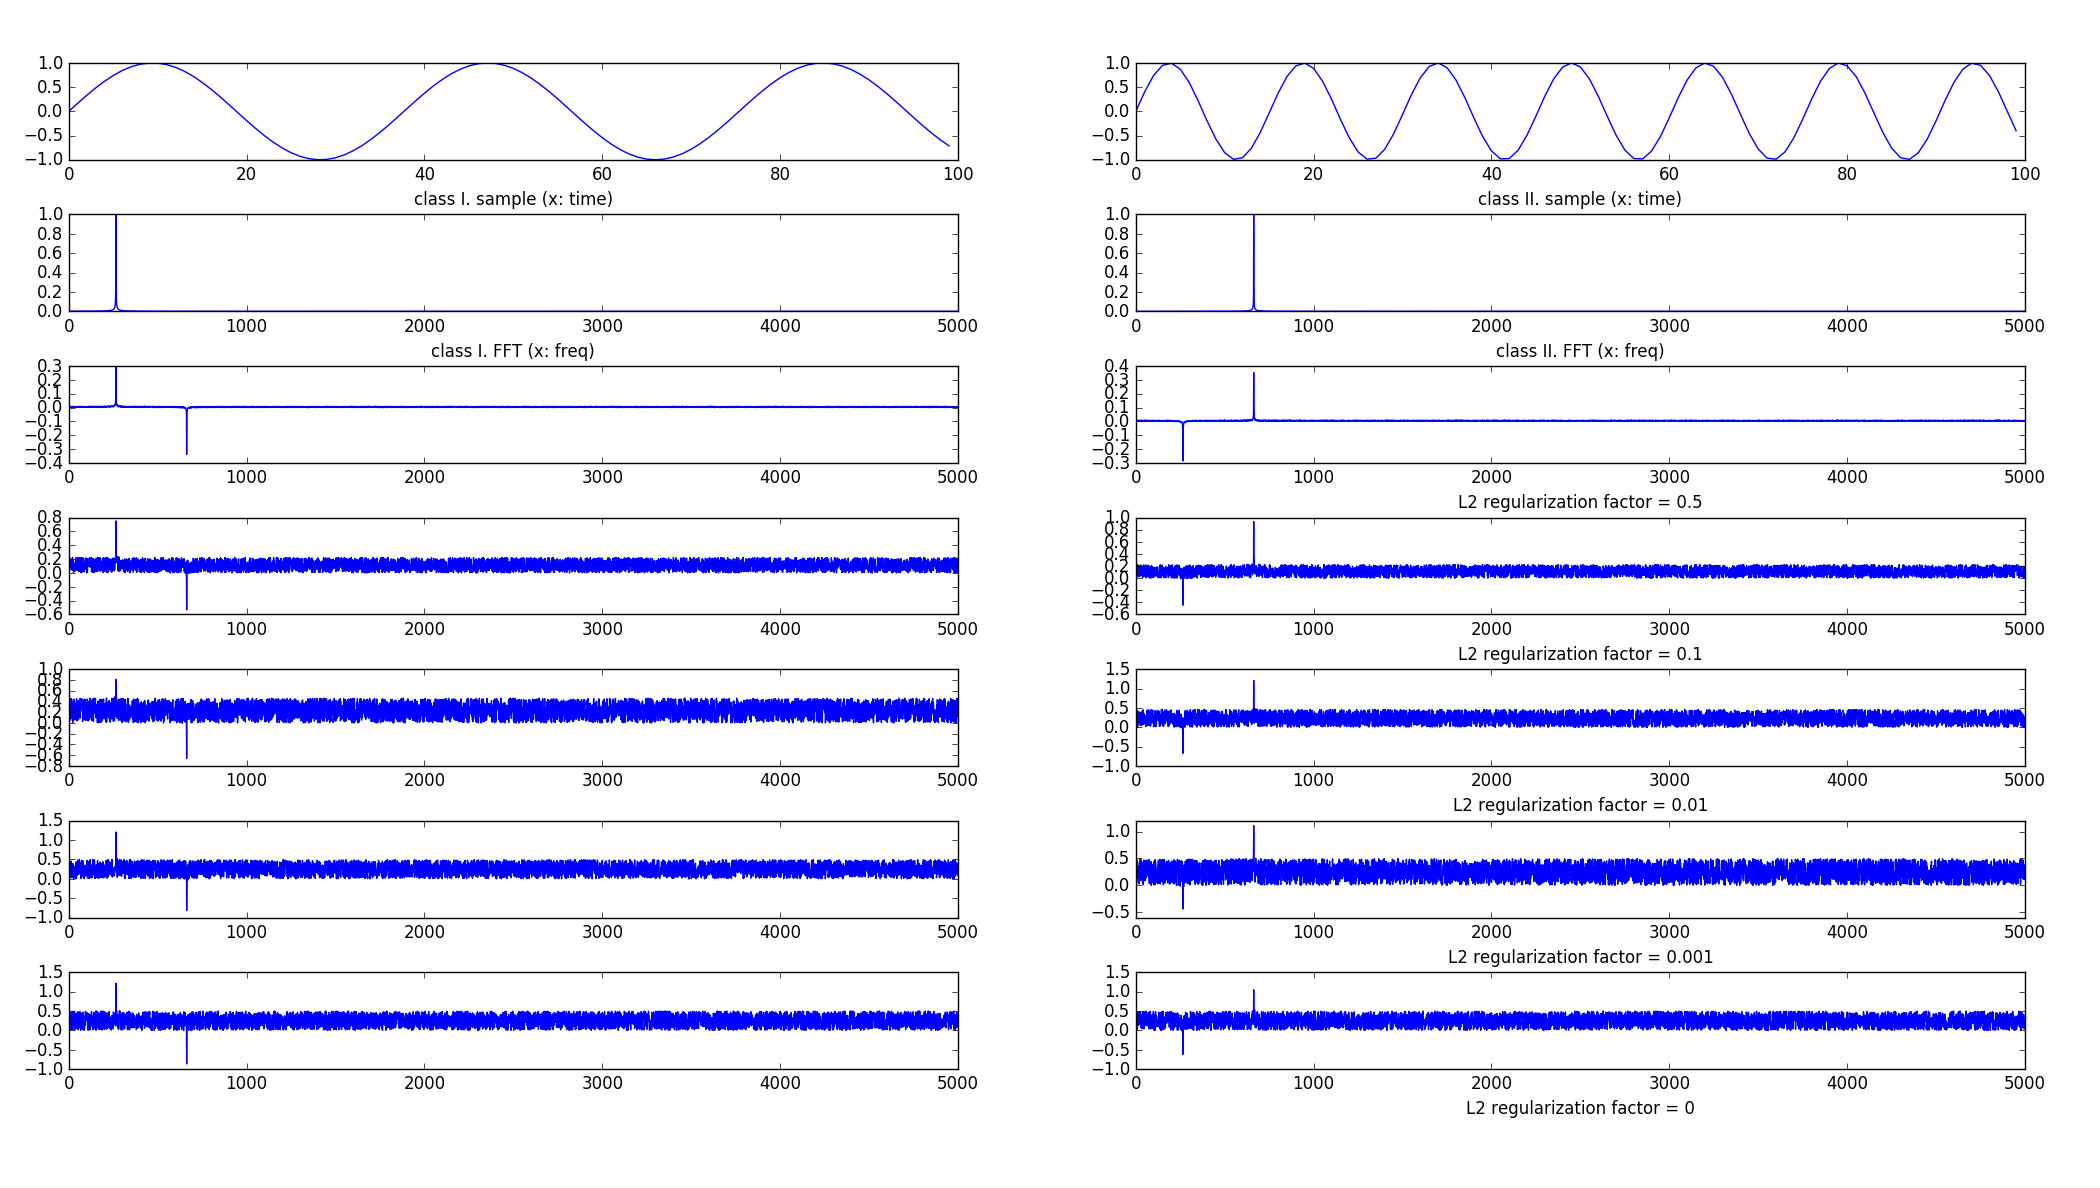
\includegraphics[width=\textwidth]{L2_factor_plot.png}
	\caption{The network was trained with the same parameters as the one depicted on \ref{fig:reg}, except that it was trained for five times longer. Despite the result is quite the same as the result achieved with greater regularization factor, overfitting should be avoided. Overfitting occurs when the network $N$ tends to perform well on the training set, but fails to recognize unmet samples, because either the training samples were not general enough, either the network was just large enough to memorize each one of the samples, or both. }
	
	\label{fig:overtrain}
\end{figure}


\paragraph{Dealing with multiple waves}
Approaching real life problems, more parallel signals should be introduced to the network. In this subsection the case of recognizing overlapping frequencies and common frequencies are examined. The networks were initialized and trained identically to the network in previous experiment with $\lambda=0.5$. In the first case six different base functions were used to compose the samples. On Figure \ref{fig:multi} it is really trivial that the network is not just capable of separating low-pitch samples from high-pitch samples, but can recognize different patterns, even if they are scattered throughout the state space of the input. In the second case the conclusion is that the perceptrons (if well trained) will look only for relevant signals and patterns in the input.  See Figure \ref{fig:multi-common}

\begin{figure}
	\centering
	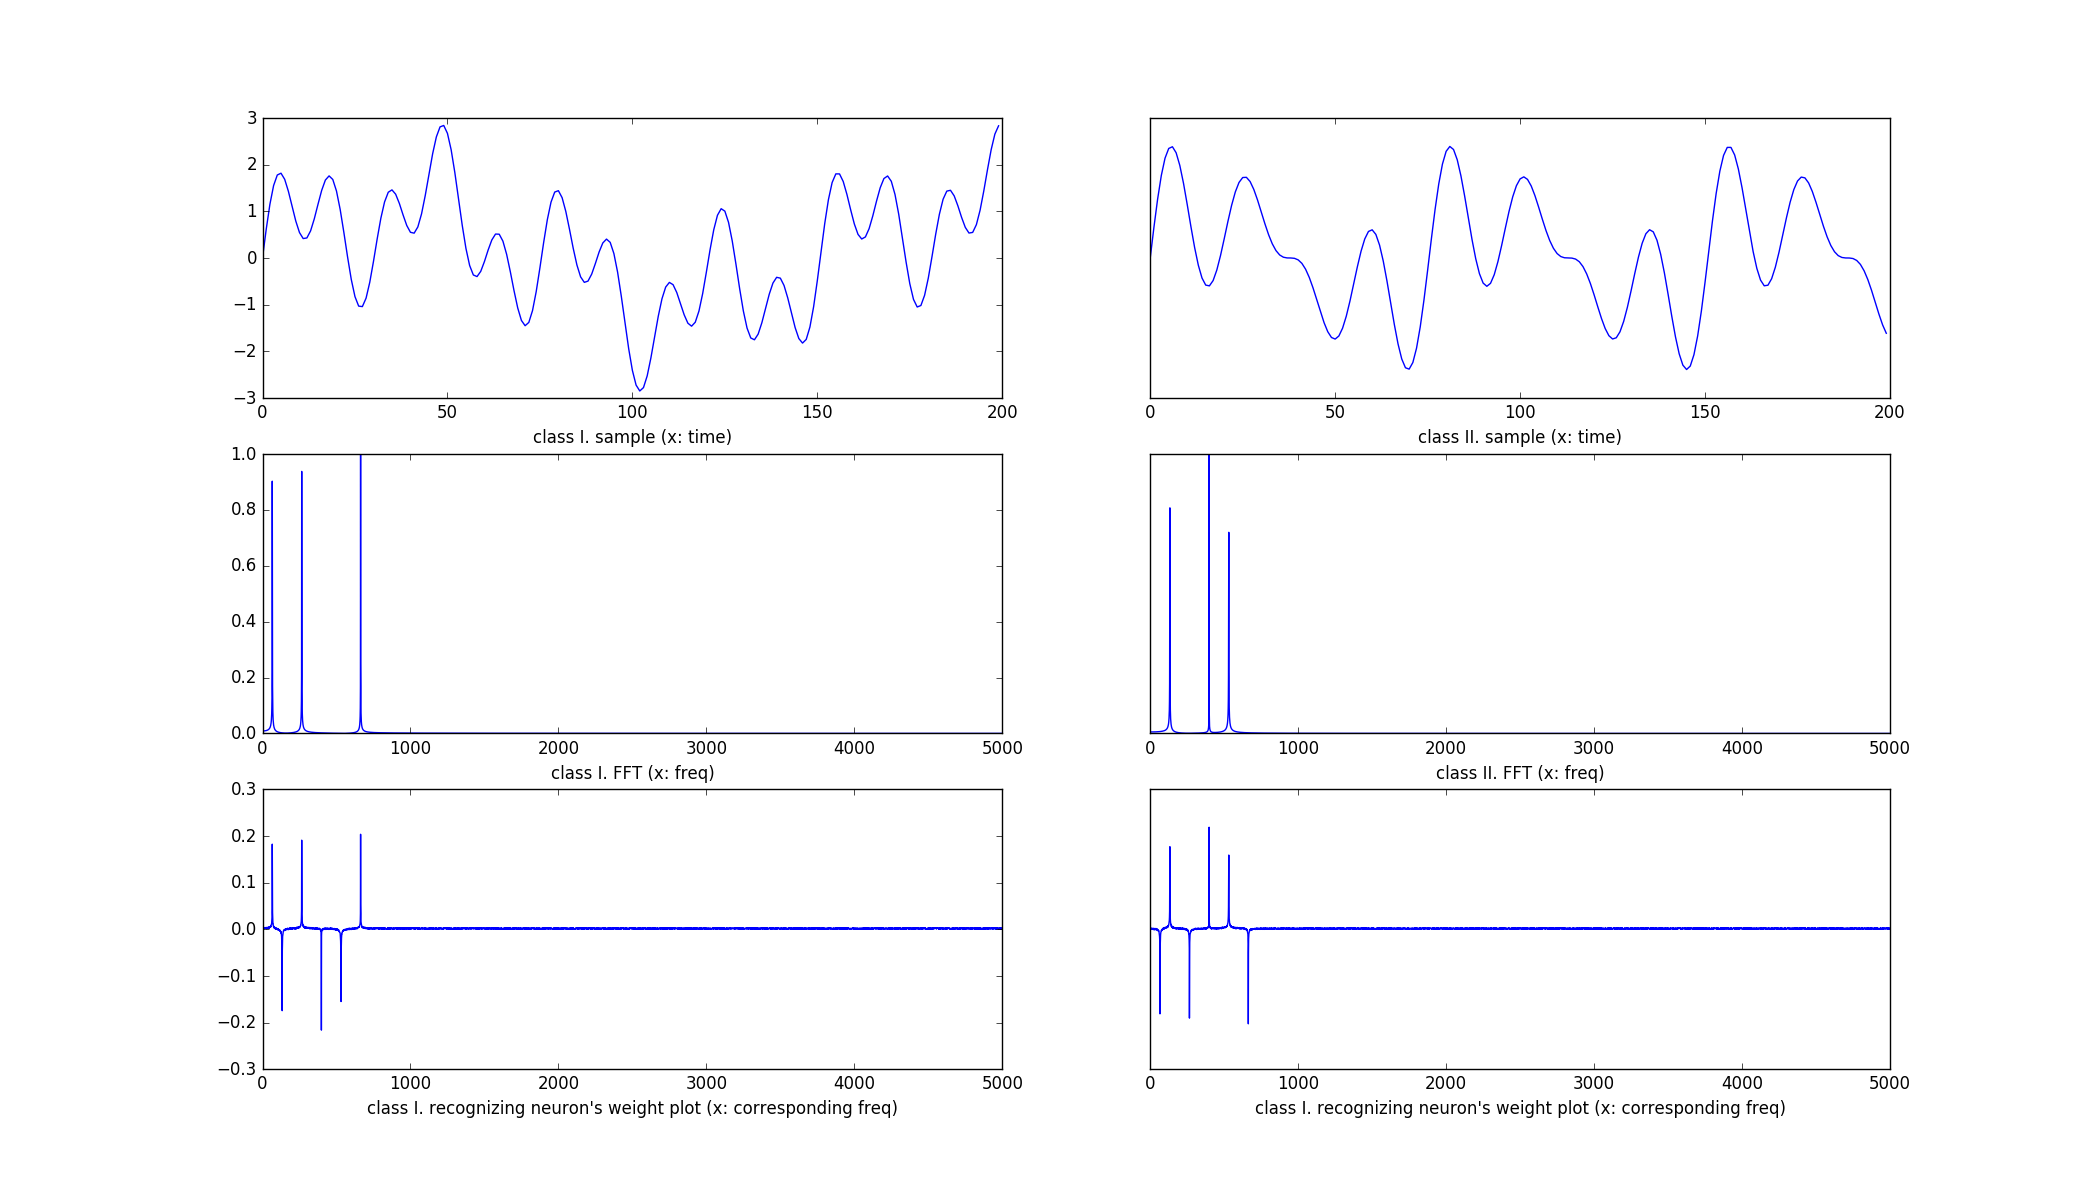
\includegraphics[width=\textwidth]{multiple---N5000---L2-5e-1.png}
	\caption{Each sample is an equal combination of 3 independent sine function. The frequency of the waves are not separated to low and high frequencies, both can be found in each sample, but it is important to notice, that the two samples do not have any common component.}
	
	\label{fig:multi}
\end{figure}


\begin{figure}
	\centering
	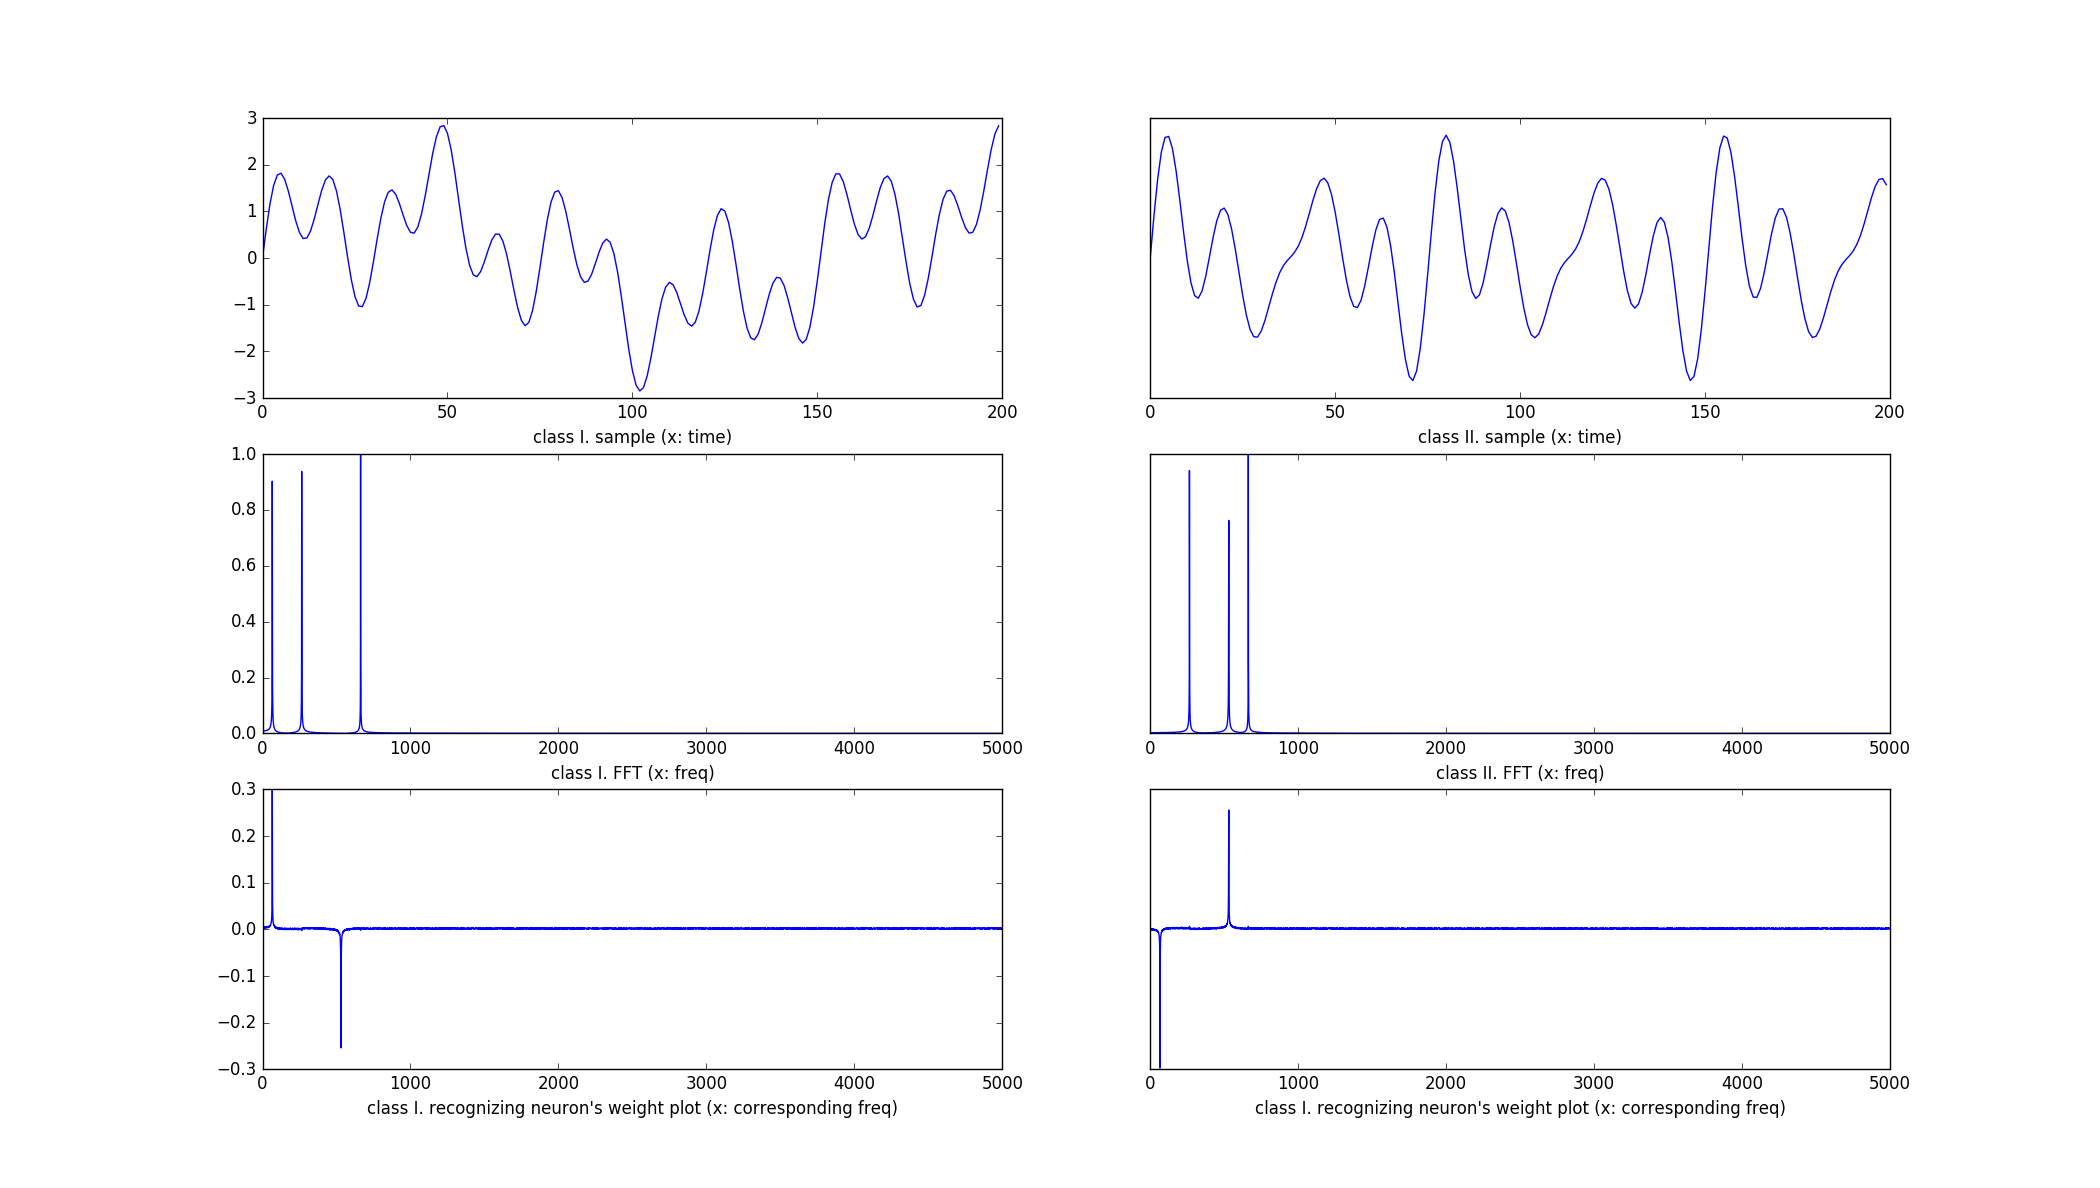
\includegraphics[width=\textwidth]{multiple--common-20-50Hz--N5000---L2-5e-1.png}
	\caption{In opposite to the case depicted on Figure \ref{fig:multi} here the samples have two common component, meaning that in the base functions there are two common frequency and only differs in one harmonics. The result is that the common features extracted by the FFT are discarded, and the perceptrons only learn the difference.}
	
	\label{fig:multi-common}
\end{figure}

\paragraph{Introducing Regularization.}
Regularization is simply a practical implementation of Occam's razor, meaning that the unimportant features of $\mathbf{x}$ will not be taken into account by the perceptron. 

On Figures \ref{fig:N500}, \ref{fig:N5000}, \ref{fig:N50} the weights were originally initialized with random Gaussian noise, but after training only the important frequencies' weights stayed significant. 
If the regularization factor is reduced the noise wouldn't disappear and the perceptron would still take irrelevant information into account. 
This phenomena is shown on Figure \ref{fig:reg}. 
However, instead of regularizing, we can \emph{over train} our networks, increasing the number of epochs, the number of times we show the same samples in the training set. 
Noise reduction via \textbf{overfit} can be seen on Figure \ref{fig:overtrain}. 

\subsection{Real Samples}
For acquiring samples from the environment the architecture should be wired to a physical sensor which will transfer signals from analog to digital. 
Practically external libraries are applied to perform the capturing. I used PyAudio. PyAudio provides Python bindings for PortAudio \cite{pham2006pyaudio}. 
The only thing remaining is to write an adapter to make the information format compatible with the network's architecture.

\paragraph{Capturing sound}
For the following experiments an algorithmic smart capturing is used, which enables us to record multiple sound waves with different length, without pressing a single key. The main idea is that the noise of the environment can be monitored, and in the background mean averaged. A practical threshold is set for recognizing significant audio inputs, where the magnitudes of the sampled waves reach the critical. After the recording starts, a fixed size time-frame will cancel out further activities of the capturing system. Another option is to end the capturing process when the magnitude of the input falls below a threshold. Either way, the samples are gathered in a list, and each of them are transformed to frequency domain with \emph{N-FFT}, producing equal length inputs  $\mathbf{x^i}$ for the network.

\paragraph{Defining the classes}
For human interpretation it is useful, that the separated classes are labeled, while from the aspect of the network it is totally irrelevant what the classes represent. That is an important thing to understand, both in supervised and in unsupervised learning. In the next cases separation sound waves of \emph{Hello} will be separated from samples of \emph{Goodbye}.

\subsection{Binary classifiers}
\paragraph{First greeting recognizer}
The first model trained on greetings and farewells is working as expected. In the demo found at \cite{DV} \url{~/demo/audio/so.py} the user is asked to input number of $N$ samples representing class I, and the same number from class II which will be labeled with the assumption that the samples do not overlap. The length of the samples can vary in time, because the smart capturing takes care of the preprocessing. 
For ending the recording session produce some loud noise, a clap should do. 
The labeled samples are then taken into account as the training set for the network, and the process adjusting the parameters begins. 
After 30 epochs of training the network waits for new $\mathbf{x}$ to classify. 
A few tests can be made to ensure the network is working well. 
My results with N=1000, on 3-3 input sample is performing around 91\% (100 tests were performed in total). 
Sending a \textbf{\textsc{sig-term}} will end the testing session and a summary window will pop up, probably something like on Figure \ref{fig:hello}.

\subsection{Multiclass classification}
\paragraph{Recognizing greetings in multiple languages}
Currently the model works like the one depicted on Figure \ref{fig:dumb}. 
A real task can be defined, where the network $\mathcal{F}$ has to classify in which language the user said hello. Unfortunately there are more languages than two, but neural networks are flexible enough to be able to recognize and separate the inputs into  $N$ number of classes. For the improved model see Figure \ref{fig:improved} 

The experiments were done with 5 different languages: \emph{French, Arabic, Spanish, German, Hungarian}. The training scene is the same as in the previous cases: input sequentially $N$ number of samples for each language, end the recording with a clap.
For a demonstration script check out \cite{DV} \url{~/demo/audio/nclass.py}.
The network trains on the given set, and the system is ready for testing.

With the following hyperparameters: 1-1 number of samples in each language, \emph{mini-batch}$=1$, \emph{number of epochs}$=15$, $\lambda=0.005$, from random Gaussian initialization a network with 60\% performance can be obtained.
\emph{Note}: at first 60\% may sound only slightly better then the 50-50 guessing, but considering the fact that the random guess would be distributed now between 5 classes, resulting in 20\% hit-rate, meaning that only every fifth greeting would be classified correctly. 
Compared to that, 60\% is much better -- the network is tells the good answer in more than half of the cases.

With larger training set, 3 samples for each language the result raised over 85\%. Comparing to industrial networks the training set used to adjust the parameters is very small in size. 
For larger projects usually the training set contains thousands and millions of samples, and overfitting is less likely to occur. 
For such a narrow network trained with a poor training set it can be said that 85\% is not that bad at all. Although the result still depends on who tests the configured network.

\begin{figure}
	\centering
	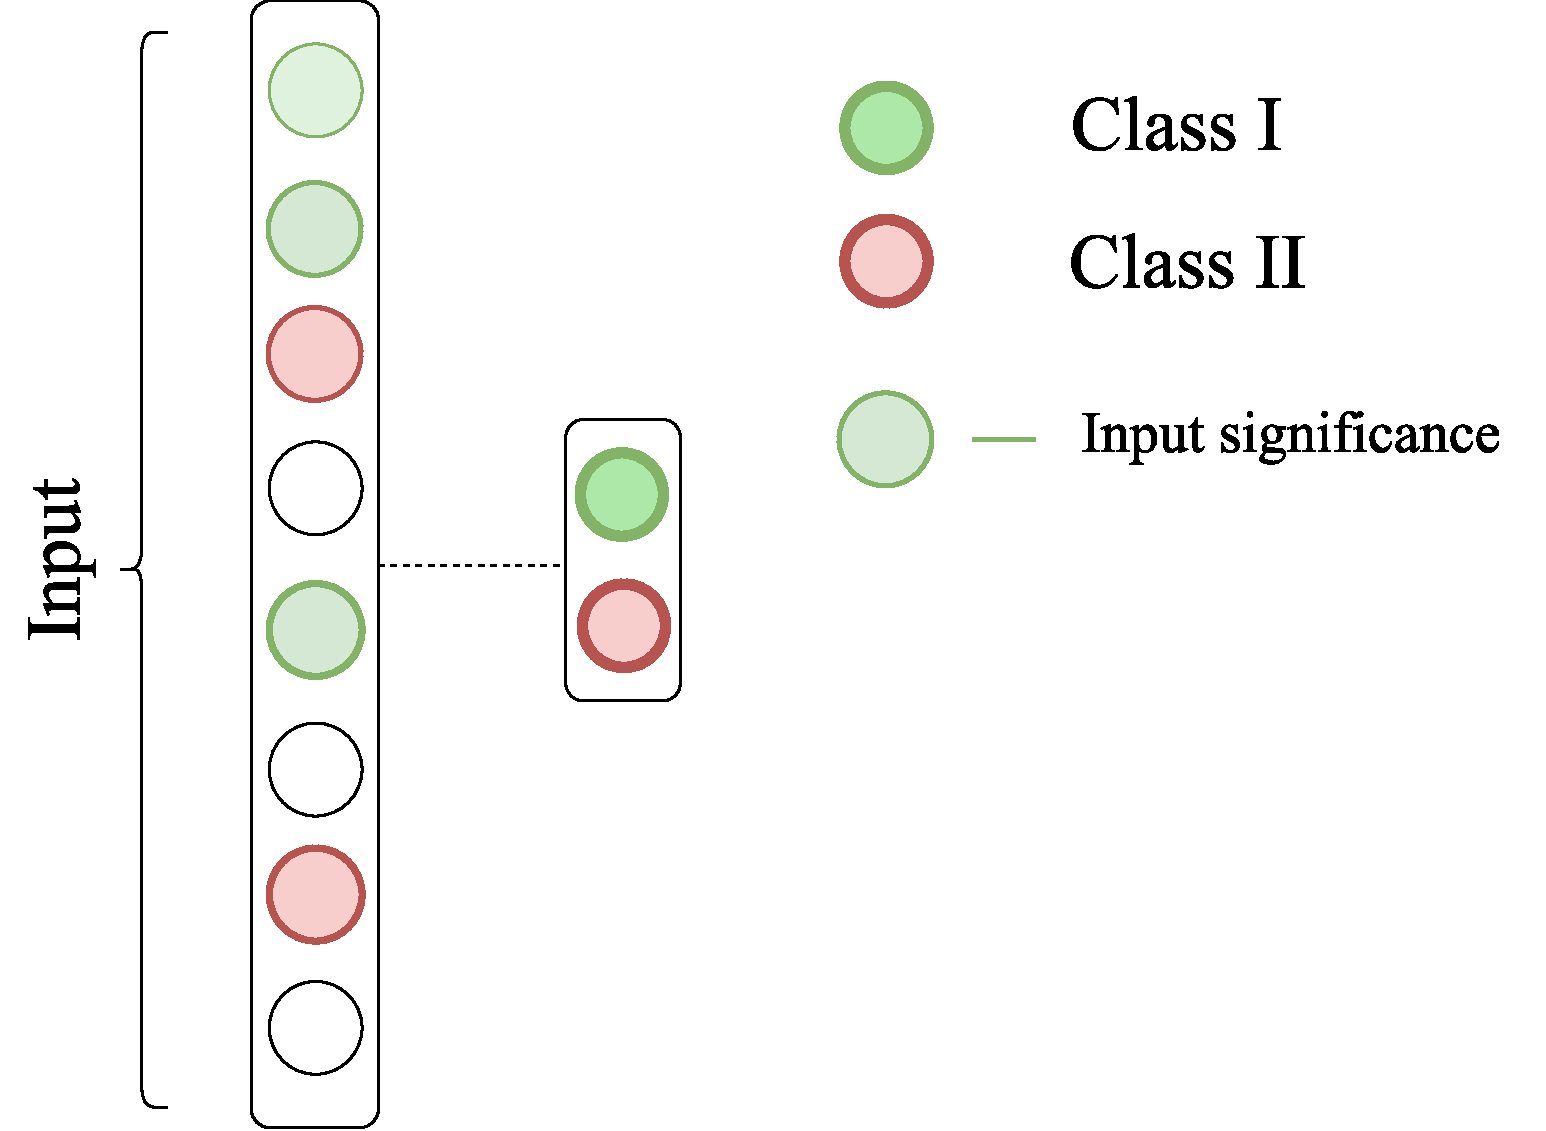
\includegraphics[width=0.5\textwidth]{current-model.pdf}
	\caption{A basic perceptron model, operating on 8 clues of the input. The perimeter of each input node describes how much it increases the output of the perceptron with the same color and decreases the neuron with opposite color. Input nodes which are not colored holds irrelevant informations for both perceptrons, therefore discarded.}
	
	\label{fig:dumb}
\end{figure}

\begin{figure}
	\centering
	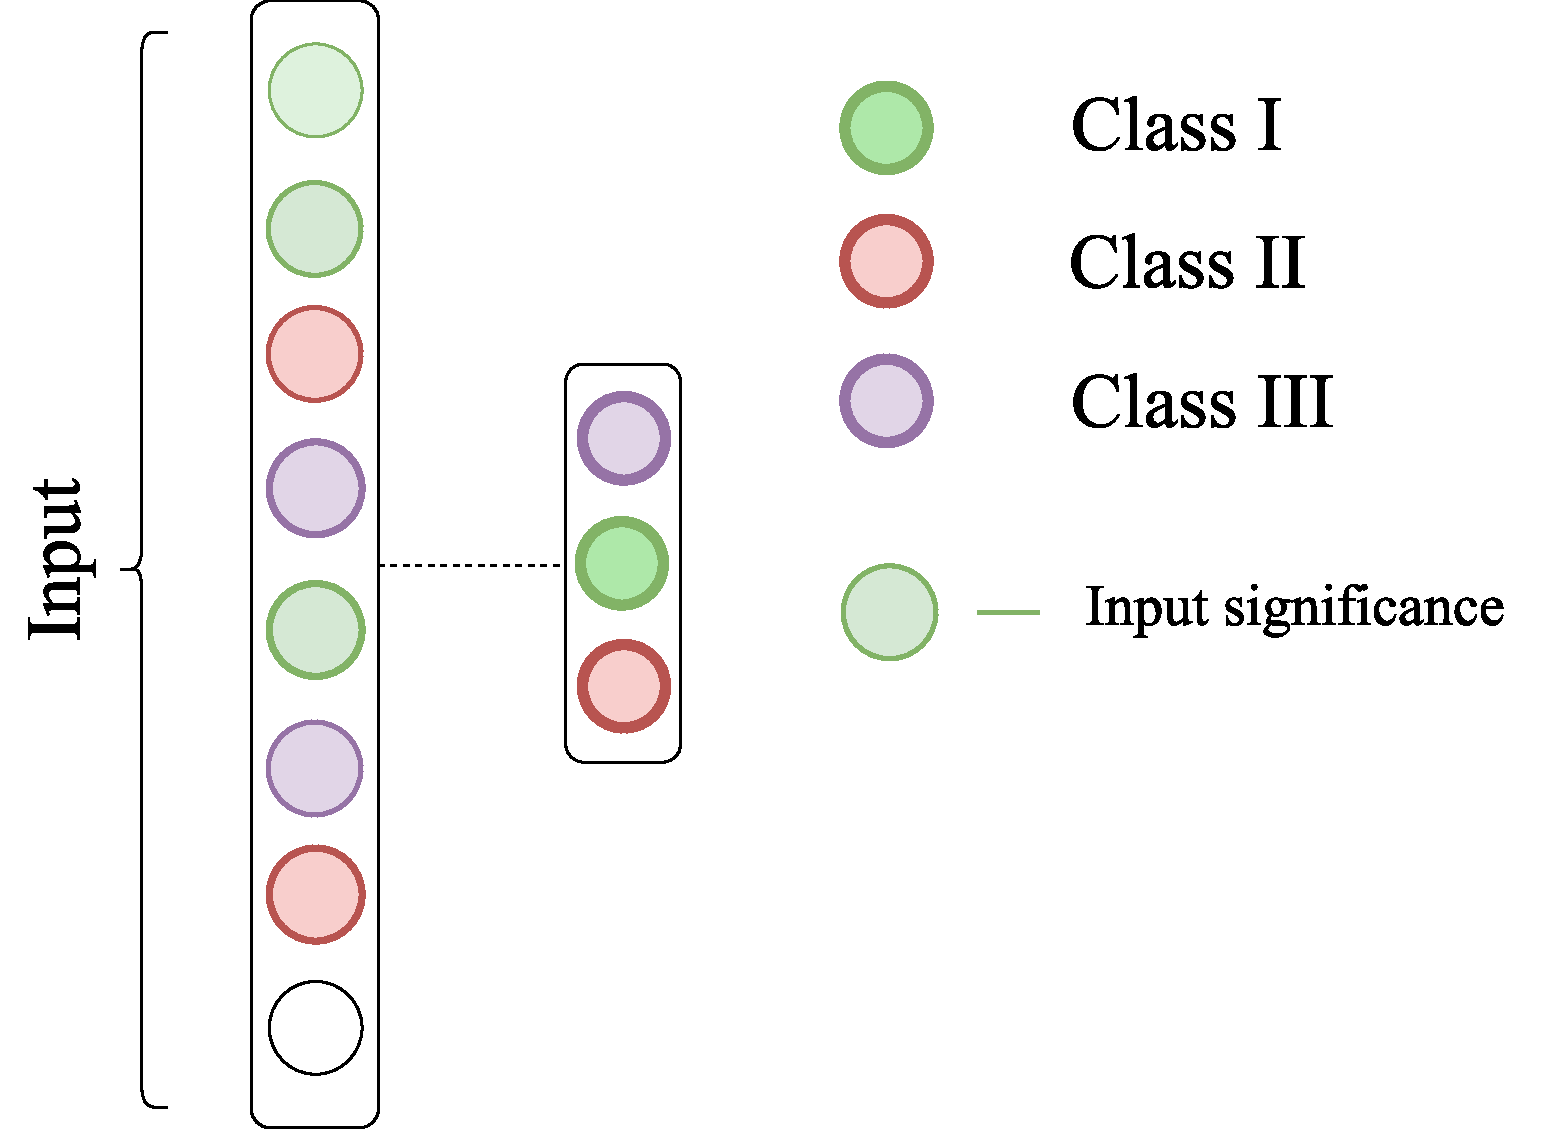
\includegraphics[width=0.5\textwidth]{improved.pdf}
	\caption{An improved perceptron model, operating on 8 clues of the input $\mathbf{x}$ , deciding which class it belongs to. The weight anti-symmetry is not so trivial in this case because perceptrons of multiple classes can be turned on by one single feature while other perceptrons are inhibited by the same feature or may even discard it. Meaning that the colors on this figure are a bit tricky, because each input node can be shared between the classes.}
	
	\label{fig:improved}
\end{figure}

\subsection{Conclusion}
So far it was shown how single layer neural networks work. 
How they should be thought of, what difficulties arises during their training. 
The capabilities of shallow networks were met during tests with the N-multiclass classifier. 
The next topic of the investigation is that how can these perceptron layers be combined to each other, 
for example to recognize whether a user said yes or no, without explicitly telling  which language he or she was speaking.

\begin{figure}
	\centering
	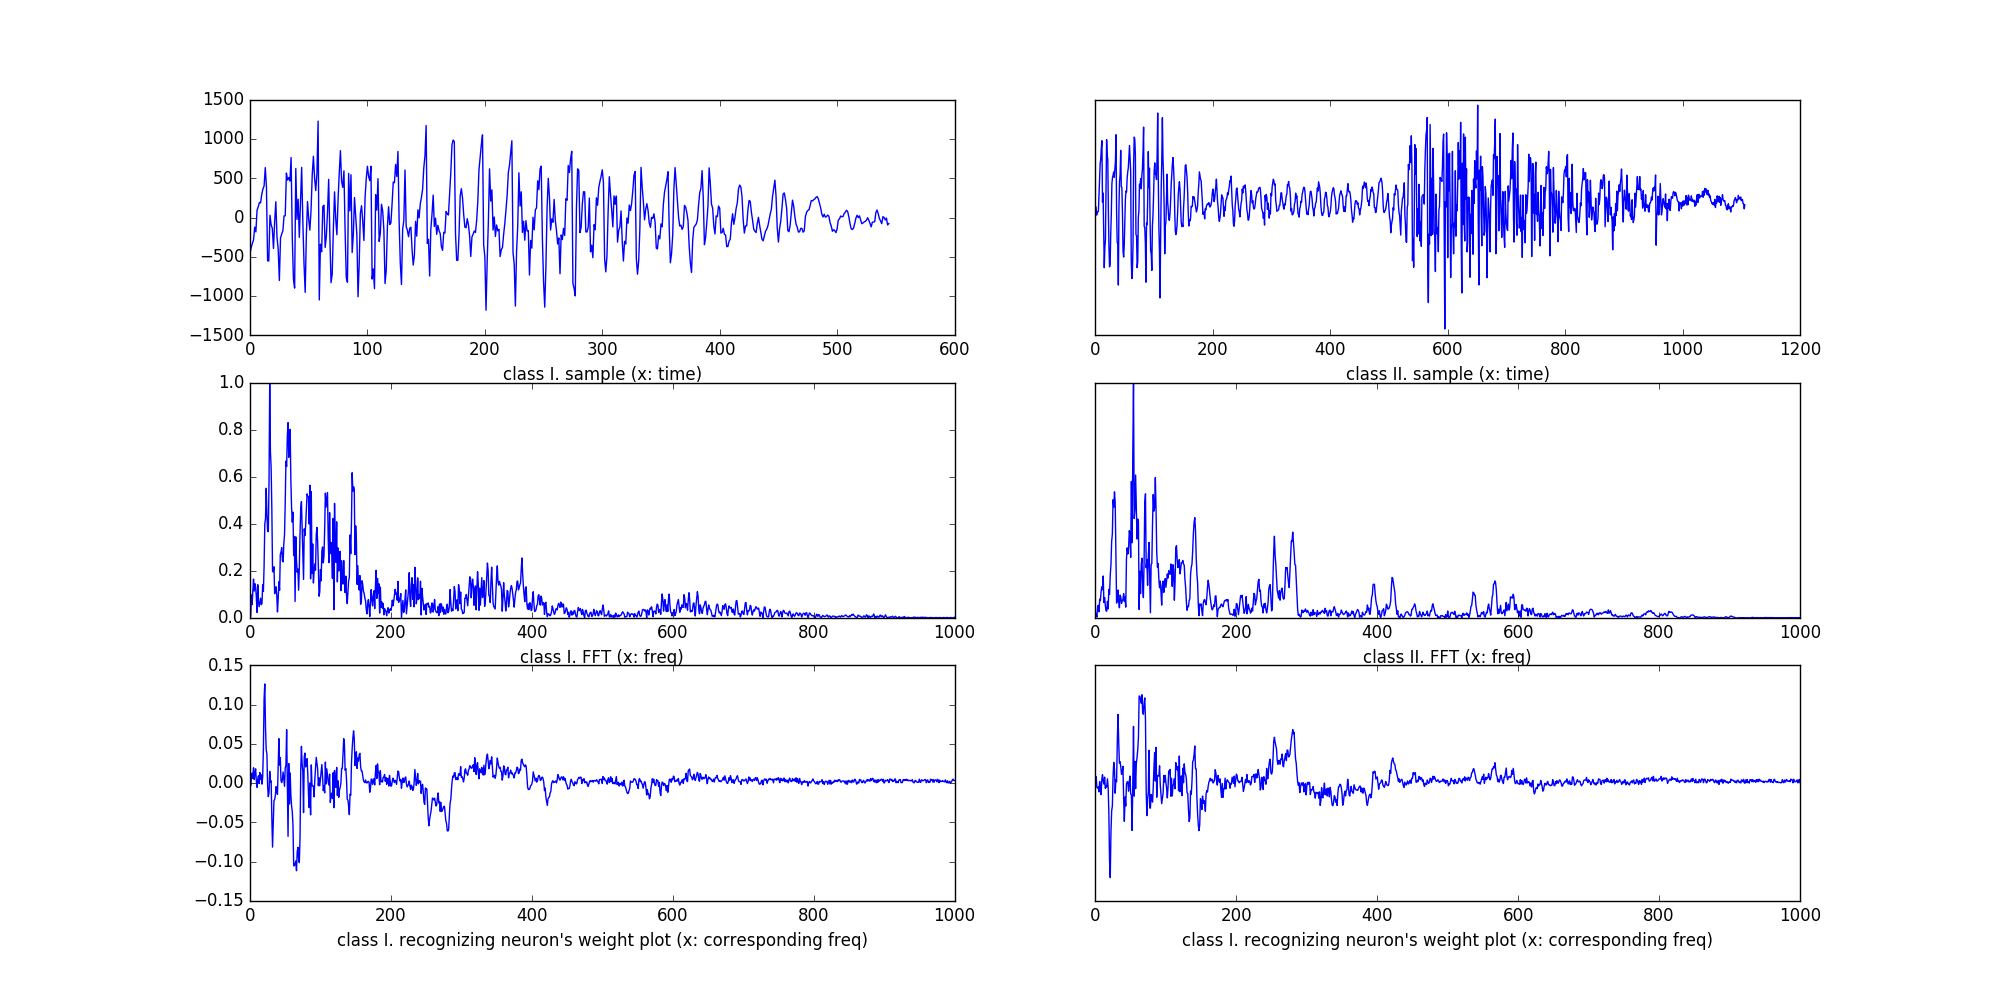
\includegraphics[width=\textwidth]{hello-goodbye-N1000-L205}
	\caption{On the left: the first example of the whole training set, showing the wave and frequency plot of a \emph{Hello}. On the right: the same for the word \emph{Goodbye}. guesses more than half 
	As experienced on Figure \ref{fig:N500}, an anti-symmetric pattern arises in the weight plot of the classifier perceptrons. 
	One pattern in the frequency domain of \emph{Goodbye} samples is very dominant and the weights of the \emph{Goodbye}-recognizing perceptron fits on it very well, while the same pattern can be found in the opposite perceptron's weight plot with negative sign.}
	
	\label{fig:hello}
\end{figure}

\begin{figure}
	\centering
	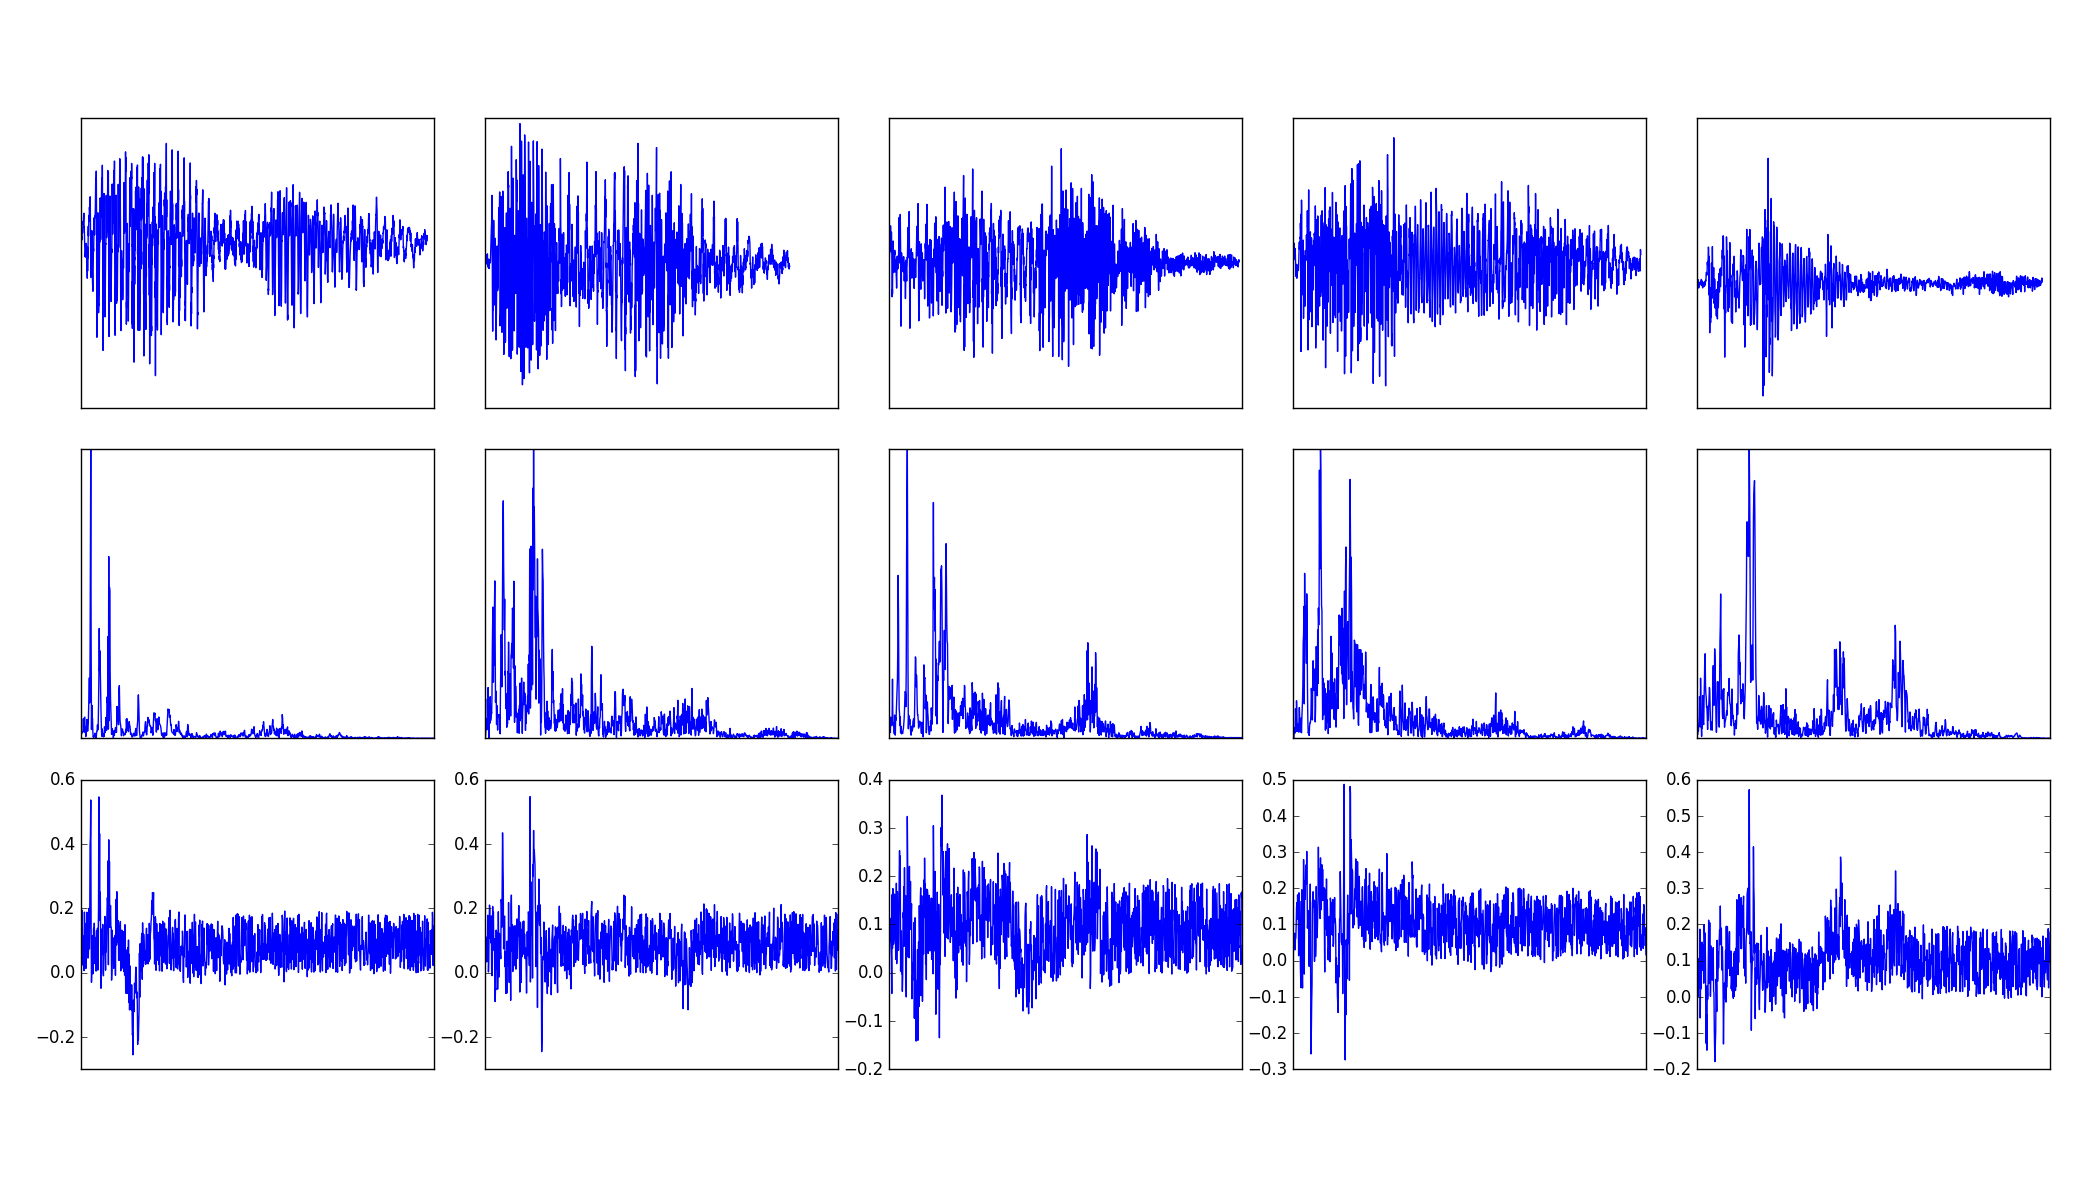
\includegraphics[width=\textwidth]{hello-5lang-3each}
	\caption{On this figure the sample time, frequency and the perceptrons' weight plots are depicted of the network that recognizes greetings in 5 languages. For human eyes it is hard to tell from either the time and frequency domain plot the corresponding language. The recorded greetings were sampled by me saying \emph{Bonjour, Salem, Hola, Halo} and \emph{Csá}}
	
	\label{fig:hello5}
\end{figure}
